\documentclass[12pt, a4paper]{article}
\usepackage[a4paper,top=2.5cm,bottom=2.5cm,left=2.5cm,right=2.5cm,marginparwidth=1.75cm]{geometry}
\usepackage{array}

% =========================
% Packages
% =========================
\usepackage{graphicx, natbib, enumitem, tabularx, ragged2e}
\usepackage[hidelinks,colorlinks=true,linkcolor=blue,citecolor=blue]{hyperref}
\usepackage{booktabs, float, parskip}
\usepackage{caption, amsmath, amsfonts}
 % for positioning
\newcolumntype{C}{>{\centering\arraybackslash}X}
\newcolumntype{L}{>{\RaggedRight\arraybackslash}X}


% =========================
%% We install packages to a) insert graphics  b) create Harvard citations c) create clickable hyperlinks respectively.  
% =========================


\title{Examining country-of-origin effects on the occupational category of migrant workers in the UK.}
\author{EC226 Assignment in Applied Econometrics - Group 12-3\\ 5510889, 5512506, 5513578, 5534070, 5550841
}
\date{April 2025}



\begin{document}

\bibliographystyle{agsm}

\maketitle

\pagebreak

% =========================
\section{Introduction} \label{sec:intro}
% =========================


%% You should give a motivation for your work and discuss the policy (or other) issues which you are trying to address. Given this context, you should then describe your detailed research question(s).

%% You should lay out the crucial parts of your argument. It is often nice to finish the introduction with a road map which tells the reader the structure of the essay and gives very brief summary of your findings.

Since 2022, immigration levels to the UK have climbed significantly  \citep{ONS2023_LTIM}. Questions arise as to whether immigrants are employed in jobs commensurate with their skills or if “brain waste” is occurring, whereby skilled workers end up in lower-skill occupations. We note a noticeable gap in literature assessing skill matching effects within the UK labour market, akin to prior analyses conducted for the United States by \citet{MattooBrainWaste}. Motivated by this gap, our study explores the question: how does an immigrant’s country of origin affect their employment within distinct skill-based occupational categories (high-skilled, medium-skilled, and low-skilled) in the UK?

Answering this question is crucial for maximising the productive potential of migrants and for informing post-Brexit immigration and labour market policies. We tested the application of self-selection migration theory, exploring how occupational outcomes of immigrants shift due to labour market expectations changes. To achieve these goals, we leverage rich data from the 2021 UK Census and control for key individual characteristics such as level of educational attainment, age, sex, and duration of stay in the UK. 

The remainder of this paper will cover the literature review, dataset summary, methodology, empirical results and the conclusion.

% =========================
\section{Literature Review} \label{sec:lit}
% =========================
A wealth of literature has examined the labour market integration of immigrants, often highlighting a mismatch between immigrants’ skills and the initial jobs. Theoretically, workers with higher human capital should attain better-paying, higher-skilled occupations \citep{BeckerHumanCap}. Empirical studies, however, have noted that foreign-acquired skills may not fully translate into host-country labour market success. Immigrants frequently experience “brain waste,” where even well-educated individuals find themselves in jobs below their qualification level. This pattern is documented by \citet{MattooBrainWaste}, studying immigrants in the United States. They show that occupational outcomes vary strikingly by country of origin among immigrants with similar education. \citet{MattooBrainWaste} attribute these disparities to origin-country attributes affecting skill transferability. Their findings suggest country of origin can be a proxy for the quality and transferability of an immigrant’s human capital. However, \citet{MattooBrainWaste}'s approach treats occupational categories as unordered, employing a multinomial logistic model does not account for the social hierarchy that is inherent in skill-levels. 

Another relevant strand of literature comes from \citet{BorjasSelfSelection}'s self-selection model of migration, which projects that the skill composition of immigrants varies systematically based on country-of-origin conditions (incentives and barriers). In high-income source countries, only individuals with higher skills and earning potential are likely to migrate given the high opportunity cost of leaving (foregoing strong home-country wages). Lower-skilled individuals from low-income nations have an incentive to migrate for better wages abroad, if they possess the necessary funds to migrate. Distance and policy-barriers can also shape migration incentives: greater distances between origin and destination countries raise the migration costs, so only those expecting large returns (high-skill individuals) might migrate. Migrants from countries with restrictive entry requirements tend to be filtered out relative to free movement regimes as well. We exploit the Brexit referendum to make inferences about the validity of this reasoning. These theories inform our choice of key explanatory variables: origin-country GDP per capita and distance from the UK to capture development and migration costs.

Empirical research on the UK aligns with other international study, while offering specific variables that are context-dependent. \citet{DustmannFabbriLanguage} show that English language proficiency has a strong positive effect on immigrants’ employment probabilities in the UK. Indeed, \citet{MattooBrainWaste} noted that immigrants from ex-British colonies achieved especially good occupational outcomes in the US, likely due to their English-medium education and other transferable credentials. 

Lastly, literature notes a U-shaped curve in immigrants’ occupational trajectories \citep{ZorluUshaped}. Immigrant workers could experience an initial occupational downgrade upon arrival, followed by upward mobility as they assimilate and acquire host-country experience \citep{ChiswickTimeSpent}. Given waves of immigration, this can result in a distribution where immigrants are over-represented at both tail ends of the skill distribution. This could mean highly educated immigrants eventually climb into the high-skilled tier, or remain stuck in low-skilled employment, creating a gap in the medium-skill range. Our research expands on such relatively under-researched phenomenon. Testable hypotheses for our empirical work are: 

\begin{enumerate}[label=(\roman*)]
    \item origin-country English and colonial ties should raise the probability of high-skill employment and lower the probability of low-skill employment
    \item higher GDP per capita and greater distance should likewise favour positive selection
    \item medium-skill outcomes should exhibit weaker or null origin effects
\end{enumerate}


% =========================
\section{Dataset Summary} \label{sec:data}
% =========================

This report focuses on the effect of migrants’ country of origin on their occupational placement in England.  The primary dataset is the 2021 UK Census, consisting of a random 5\% sample of person-records from Census 2021 for England and Wales.  We then merged these microdata with two country-level series from the World Bank: GDP per capita and tertiary-education expenditure (as a percentage of GDP).  To fill a gap for Nigeria, we interpolated Cameroon’s and Ghana’s tertiary-education figures from the World Bank and extrapolated a plausible value (see Appendix~\ref{tab:secondstagetert}).  Finally, we appended bilateral distances from the CEPII dataset, measured in great-circle kilometers from each origin country to the UK.

Our full sample contains 3{,}021{,}455 persons.  Restricting to individuals who were employed at the time of the census and aged between 25 and 65 yields 993{,}034 observations, covering 17 origin countries across five continents.  All further analysis uses this working sample.  Because Census geography only reports 17 distinct birth–country codes, our key origin variable is limited accordingly.  We also constructed three binary indicators for subsample analysis: 
\begin{itemize}
  \item \texttt{sex} (male/female),
  \item \texttt{uk\_born} (UK-born vs.\ foreign-born),
  \item \texttt{brexit\_cohort} (arrival pre-2016 vs.\ post-2016).
\end{itemize}

Two additional covariates—\texttt{colonies\_post\_1945} (1 if the origin state was a British colony in 1945, 0 otherwise) and \texttt{home\_eng} (1 if English is the primary official language, 0 else)—were coded manually from historical and institutional sources.

In the probit models discussed below, we always control for age; country of birth (including the UK as its own category); English region of residence; years spent in the UK; and highest qualification level.

Our dependent variable, \texttt{hrp\_ns\_sec\_grouped}, collapses the detailed NS-SEC categories into three ordered groups:
\[
  \underbrace{\text{High}}_{\texttt{hrp\_ns\_sec\_grouped}=1},\quad
  \underbrace{\text{Medium}}_{\texttt{hrp\_ns\_sec\_grouped}=2},\quad
  \underbrace{\text{Low}}_{\texttt{hrp\_ns\_sec\_grouped}=3}. \quad
\]
(See Table~\ref{tab:variables} for the exact mapping.)

Motivated by the literature, we include five key country–level regressors:
\texttt{lgdp\_per\_capita\_2021}, \texttt{migration\_distance}, \texttt{colonies\_post\_1945}, \texttt{tert\_exp\_latest}, and \texttt{english\_main\_language}.  
\begin{itemize}
  \item \texttt{lgdp\_per\_capita\_2021} and \texttt{migration\_distance} (in km) control for economic development and geographic proximity.  
  \item \texttt{colonies\_post\_1945} flags a state’s colonial status as of 1945.  
  \item \texttt{tert\_exp\_latest} is the share of GDP spent on tertiary education in 2021.  
  \item \texttt{home\_eng} equals 1 if English is the official medium of instruction, 0 otherwise.  In our sample, roughly 57.9,\% of respondents come from an English-language origin country.  
\end{itemize}

Summary statistics and further description of these control variables appear in Appendix~\ref{tab:variables} and ~\ref{tab: sum stat}.

\section{Methodology}  

\subsection{Ordered Probit Model:}\label{probit}
% =========================
To address the categorical nature of individuals’ occupational placement, previous studies have made use of a multinomial logit model. Our study builds on this through a ranked probit to respect this implicit ranking. In the model, we included 3 independent variables, where we follow \citet{MattooBrainWaste}'s assumptions. We have 17 dummies for the Country of Birth (including the UK) for immigrants and locals. The model includes categorical variables highes\_qualification (7 dummies, 0-6) and region\_num (9 dummies, 1-9), along with the controlled continuous variables age, age squared, and time spent in the UK to estimate the marginal country level effects for high, medium, and low skilled workers separately. Details regarding the controlled variables are covered in details in the Appendix. UK born were used as the baseline category, and we take male-only observations (females will be considered in section 4.3). 

We let the observed skill variable 
\[
  \text{hrp\_ns\_sec\_grouped}_i \;\in\;\{1\, (\text{high}),\,2\ (\text{medium}),\,3\ (\text{low})\},
\]
The Ordered Probit Model (1) is as follows:
\[
  \Pr\bigl(\text{hrp\_ns\_sec\_grouped}_i = j \mid X_i \bigr)
  \;=\;\Phi\bigl(\alpha_j + X_i'\beta\bigr)
  \;-\;\Phi\bigl(\alpha_{j-1} + X_i'\beta\bigr),
  \quad j=1,2,3,
\]
where:
\begin{equation}\label{eq:probit}
\begin{align*}
X_i' \beta &= \sum_{c=2}^{17} \beta_{c} \mathbb{1}\{\mathrm{country\_of\_birth\_25a}_i = c\} 
           + \sum_{q=1}^{6} \gamma_{q} \mathbb{1}\{\mathrm{highest\_qualification}_i = q\} \\
           &+ \sum_{r=2}^{9} \delta_{r} \mathbb{1}\{\mathrm{region\_num}_i = r\} 
           + \theta_1 \text{age}_i 
           + \theta_2 \text{agesq}_i 
           + \theta_3 \text{time\_spent\_in\_uk}_i,
\end{align*}
\end{equation}

and the two cut‐points satisfy 
\(\alpha_0=-\infty<\alpha_1<\alpha_2<\alpha_3=+\infty\).

The first‐stage ordered probit yields country‐specific \emph{marginal} effects for high, medium, and low occupational placement. 


\subsection{Multinomial Logit Model}

In order to compare our model to models used in previous literature, we employ a multinomial logistic regression similar to that employed by \citet{MattooBrainWaste}. The model takes the form:
\begin{equation}\label{eq:mlogit}
  \Pr(y_i = j \mid X_i)
  \;=\;
  \frac{\exp\bigl(X_i'\,\beta_j \bigr)}%
       {\sum_{k=\{\text{high},\text{med},\text{low}\}}
              \exp\bigl(X_i'\,\beta_k\bigr)}\,,
  \quad j\in\{\text{high},\,\text{med},\,\text{low}\}\,,
\end{equation}


\subsection{Second Stage OLS Regression}

\paragraph{Basis Model:}
We ran multiple Ordinary Least Squares (OLS) Regressions in second stage to estimate the effect for our explanatory variables. We identified that GDP per capita and Migration Distance have the strongest link with the job skill level from \citet{BorjasSelfSelection} and \citet{MattooBrainWaste}. Therefore, our base model has these two explanatory variables to start with, and takes the form: 
\begin{equation}\label{eq:ols-base}
  y_i
  \;=\;
  \alpha
  + \beta_{1}\,\text{lgdp\_per\_capita\_2021}_i
  + \beta_{2}\,\text{migration\_distance}_i
  + \varepsilon_i,
\end{equation}
where
\begin{itemize}
  \item $y_i$ is the skill score (high=1, medium=2, low=3) for individual~$i$,
  \item $\texttt{lgdp\_per\_capita\_2021}$ is the natural log of GDP per capita of country~$i$’s origin,
  \item $\texttt{migration\_distance}$ is the bilateral migration distance (in thousands of km),
  \item $\varepsilon_i$ is an iid error term.
\end{itemize}

\paragraph{Model Extensions \& Link Tests:}
 We further run the \texttt{linktest}, \texttt{estat ovtest} (to test for omitted variables and any source of misspecification). VIF tests were conducted to test for correlation between the explanatory variables. Robust standard errors control for possible heteroscedasticity. Results show that with Log GDP per capita and Migration Distance as explanatory variables are appropriate, confirming the second stage OLS regression (3).

\paragraph{Additional Explantory Variables}
As motivated by \citet{MattooBrainWaste} and \citet{LindleyUKOverEd}, we then attempt to include a third explanatory variable that might further explain the difference in probabilities. However, our sample size was limited by the detailedness of the UK Census. After merging of datasets, we are left with 17 different countries (including the UK), which poses small sample bias and reduces statistical power to our results. To build up our model, we ran the new model with tertiary education expenditure, colonial ties, and English as the medium of instruction in home country respectively. Thus our specifications become

\begin{align}
  \text{Spec (4):}\quad
  y_i &= \alpha + \beta_1\,\text{lgdp\_per\_capita\_2021}
           + \beta_2\,\text{migration\_distance}_i \\
           + \beta_3\,\text{tert\_exp\_latest}_i  + \varepsilon_i,
           \notag\\
  \text{Spec (5):}\quad
  y_i &= \alpha + \beta_1\,\text{lgdp\_per\_capita\_2021}
           + \beta_2\,{migration\_distance}_i\\
           + \beta_4\,\text{colonies\_post\_1945}_i + \varepsilon_i,
           \label{eq:ols-extended}\\        
  \text{Spec (6):}\quad
  y_i &= \alpha + \beta_1\,\ln(\text{GDPpc}_i)
           + \beta_2\,{migration\_distance}_i
           + \beta_5\,\text{home\_english}_i + \varepsilon_i., 
           \notag
\end{align}

In turn, we performed the \texttt{linktest}, \texttt{ovtest} (Ramsey RESET), and heteroskedasticity checks on each specification.  We find:
\begin{itemize}
  \item $\text{tert\_exp\_latest}$ and $\text{colonies\_post\_1945}_i$ fail to improve fit or significance,
  \item $\text{HomeEng}_i$ enters with $p<0.10$ for the “high” and “low” skill outcomes,
  \item No severe heteroskedasticity remains after robust (Huber–White) standard errors.
\end{itemize}
Accordingly, the baseline model \eqref{eq:ols-base} remains our preferred specification.

\paragraph{Interpretation:}
The OLS coefficients $\beta_{1},\beta_{2}$ measure the partial effect of a 1\% rise in GDP per capita and a 1,000 km increase in migration distance (respectively) on occupational skill ranking.  Log‐transforming GDP captures proportional differences across high‐ versus low‐income origin countries, while migration distance controls for diaspora networks and relocation costs.

\bigskip
\subsection{Subgroup Probit Models}
  Intending to examine on policy effects brought by Brexit, we broke down our sample into Pre- and Post-Brexit immigrants with our binary variable \text{brexit\_cohort}. We ran the probit model separately for \text{brexit\_cohort} values taking “1” and “0” to estimate the country effects.

As we are aware of the immigrants’ gender difference in terms of the job skill level, as stated by \citet{AdseraGender}. We rerun model (1) for women to compute the margins, comparing with the male cohort. 

\section{Empirical Results} \label{sec:emp}

 The marginal effects from our baseline probit (N=516 746) show that high-skill probabilities are highest for the U.S. (+0.352 pp), Canada (+0.311), France (+0.303), South Africa (+0.294) and lowest for Poland (+0.060), Bangladesh (+0.074) and Portugal (+0.139).  Medium-skill effects cluster tightly around +0.38–0.40 pp, while low-skill risks peak above +0.60 pp for Poland (+0.696) and Bangladesh (+0.655) but remain under +0.30 pp for Western origins. 
 
In the baseline probit model, a 1\% increase in origin-country GDP per capita raises the probability of migrants entering high-skill occupations by 0.036 p.p. (p$<$0.01) and reduces low-skill likelihood by 0.044 p.p. (p$<$0.05), while each 1\% increase in migration distance to the UK boosts high-skill probability by 0.100 p.p. (p$<$0.01) and cuts low-skill by 0.126 p.p. (p$<$0.01).  Introducing tertiary-education expenditure has virtually no effect but when adding colonial-status, the GDP effect on high-skill more than doubles to 0.093 p.p. (p$<$0.01) and the colony dummy itself predicts a 0.183 p.p. higher high-skill probability (p$<$0.05) and a 0.235 p.p. lower low-skill probability (p$<$0.10).  Finally, allowing for home-language status confirms that English-speaking origins see a 0.089 p.p. boost into high-skill work (p$<$0.10), with GDP and distance remaining highly significant in the same directions. Across all models, medium-skill margins are statistically indistinct, highlighting potential historical and linguistic ties for shaping migrants’ occupational outcomes.

Table 11 presents average marginal effects from the multinomial logit model, Consistent with the probit results, migrants from the United States (+0.324 p.p.) and Canada (+0.310 p.p.) exhibit positive shifts into high-skill roles, followed by France (+0.300 p.p.), Germany (+0.260 p.p.), and South Africa (+0.279 p.p.), whereas those from Poland (+0.068 p.p.) and Bangladesh (+0.076 p.p.) show minimal gains. For Medium-skill effects, Poland (+0.222 p.p.) and Bangladesh (+0.270 p.p.) are lying noticeably below the mean. In the low-skill margin, Poland (+0.710 p.p.), Pakistan (+0.613 p.p.), and Bangladesh (+0.655 p.p.) see the highest increases. Whereas Western origins (United States +0.210 p.p., Canada +0.302 p.p., France +0.303 p.p.) face much smaller low-skill risks. 

To gauge how entry conditions shifted around Brexit, Table 14 and 15 show re-estimates of our multinomial logit separately for pre-Brexit (N = 506,608) and post-Brexit (N = 462,204). High-skill probabilities increase after 2016: Canada jumps from +0.298 to +0.600 p.p., the U.S. +0.334→+0.584, and Germany +0.247→+0.582. Low-skill risks fall in tandem (e.g. Canada +0.302→+0.095, U.S. +0.268→+0.102). Medium-skill effects drift downward for Western origins (U.S. +0.398→+0.314; Canada +0.400→+0.305) but edge up for Eastern and non-EU countries (Poland +0.248→+0.364; Nigeria +0.331→+0.403). These shifts suggest that post-Brexit migrants, especially from ex-British colonies, generally find stronger pathways into high-skill employment and lower barriers into lower skill employment as found by \citet{MattooBrainWaste}.


Finally, Table 16 replicates the baseline logit with the women-only subsample (N = 476,288). Rankings remain unchanged as U.S. and Canada lead high-skill probabilities again while Medium-skill margins again mostly hover near +0.40 p.p. for most groups. Low-skill risks peak among Poland (+0.610 p.p.) and Jamaica (+0.546 p.p.), and for Western origins (U.S. +0.238 p.p., France +0.287 p.p.). Close alignment with previous results confirm that origin-driven occupational disparities persist strongly among female migrants.

\section{Conclusion} \label{sec:conc}

Our research reveals that the country of origin of a migrant can impact a migrant's occupational skill level in the UK. The results show substantial heterogeneity across the countries of migrant origin, which remains unchanged even after controlling for qualifications, age, region, and time spent in the UK. Trends were also found where higher predicted probabilities of being in a high-skilled occupation are seen with migrants from higher-income countries and closer proximity to the UK. Findings suggest that supporting language training for non‐English‐speaking migrants could meaningfully aid their transition into higher occupations.

We analysed that Brexit has affected migrants' occupational categories. The probit model finds a decline in the predicted probabilities of high-skilled occupations for European migrants post-Brexit and no change for non-Europeans. Next, we observe that women tend to have lower probabilities for high-skilled employment across most country groups. However, the trends for men and women by origin country are relatively similar. 

The results are consistent with pre-existing literature on the U-shaped nature of migrants' occupational trajectories. These findings could be further expanded if we could establish the causality between origin country and occupational categories. This will account for institutional factors that might affect the labour market. The country-level predictors may not fully account for more nuanced structural inequalities like discrimination and any informal labour networks.




\clearpage
\bibliography{References}



\appendix

\section{Tables}

\subsection{Description of Variables} \label{tab:variables}
\begin{table}[H]
\small
\centering
\begin{tabular}{|p{5cm}|p{8cm}|p{3cm}|}
\hline
\textbf{Variable} & \textbf{Description} & \textbf{Source} \\
\hline
country\_of\_birth\_25a & Categorical: Country of birth grouped into 25 categories (Europe, Africa, Americas, etc.) & 2021 Census \\
\hline
region\_num & 
\begin{tabular}[t]{@{}l@{}}
Categorical: Region of residence in England\\ Values: \\
1 = North East\\
2 = North West\\
3 = Yorkshire and The Humber\\
4 = East Midlands\\
5 = West Midlands\\
6 = East of England\\
7 = London\\
8 = South East\\
9 = South West
\end{tabular} &
2021 Census \\
\hline
resident\_age\_74m & Continuous: Age of respondent in years & 2021 Census \\
\hline
age\_sq & Age squared (age\(^2\)) for non-linear effects & Created in code \\
\hline
highest\_qualification &
\begin{tabular}[t]{@{}l@{}}
Categorical: Highest qualification level achieved. \\
0 = No qualifications \\
1 = Level 1: 1–4 GCSEs or equivalent \\
2 = Level 2: 5+ GCSEs or equivalent \\
3 = Apprenticeship \\
4 = Level 3: A-levels or equivalent \\
5 = Level 4+: Degree (BA, MA, PhD) \\
6 = Other: vocational or work-based training
\end{tabular} &
2021 Census \\
\hline
sex & Categorical: Gender of respondent (1 = female, 2 = male) & 2021 Census \\
\hline
year\_arrival\_uk & Year of arrival in the UK (categorical bands) & 2021 Census \\
\hline
economic\_activity\_status\_17m & Employment status of respondent & 2021 Census \\
\hline
home\_english & Categorical: English language proficiency (main language or ability) & 2021 Census \\
\hline
how migration\_distance & Continuous: Migration distance from country of birth to UK (km) & CEPII Distance Database \\
\hline
gdp\_per\_capita\_2021 & Continuous: GDP per capita in 2021 (current US\$) & World Bank \\
\hline
colonies\_post\_1945 & Dummy: Former British colony status post-1945 (0/1) & Manually coded \\
\hline
time\_spent\_in\_uk & Continuous: Estimated years lived in UK & Derived from census data \\
\hline
uk\_born & Dummy: UK-born vs. foreign-born (0/1) & Derived from census data \\
\hline
brexit\_cohort & Dummy: Pre-Brexit vs. Post-Brexit migrant (0/1) & Derived from census data \\
\hline
hrp\_ns\_sec\_grouped & Categorical: NS-SEC grouped into Low (1-3), Medium (4-7) and High (8-14) levels & Derived from census data \\
\hline
lgdp\_per\_capita\_2021 & Log-transformed GDP per capita (natural log) & World Bank \\
\hline
{tert\_exp\_latest} & Government expenditure on tertiary education, expressed as \% of national GDP, most recent available year (2021) & World Bank \\
\hline
\end{tabular}

\end{table}

\subsection {Summary Statistics for Control Variables} \label{tab: sum stat}

\begin{table}[H]\centering
\def\sym#1{\ifmmode^{#1}\else\(^{#1}\)\fi}
\begin{tabularx}{\textwidth}{@{}lCCC@{}}
\hline\hline
                    &           b&         pct\\
\hline
Foreign-born        &            &            \\
High-Skill          &       29380&     2.95861\\
Medium-Skill        &       35479&    3.572788\\
Low-Skill           &       56300&    5.669494\\
Total               &      121159&    12.20089\\
\hline
UK-born             &            &            \\
High-Skill          &      186692&    18.80016\\
Medium-Skill        &      326951&    32.92445\\
Low-Skill           &      358232&    36.07449\\
Total               &      871875&    87.79911\\
\hline
Total               &            &            \\
High-Skill          &      216072&    21.75877\\
Medium-Skill        &      362430&    36.49724\\
Low-Skill           &      414532&    41.74399\\
Total               &      993034&         100\\
\hline\hline
\end{tabularx} \\
  \caption{hrp\_ns\_sec\_ordered by Birth Origin}
\end{table}

\begin{table}[H]\centering
\def\sym#1{\ifmmode^{#1}\else\(^{#1}\)\fi}
\begin{tabularx}{\textwidth}{@{}lCCC@{}}
\hline\hline
                    &           b&         pct\\
\hline
North East           &       46803&    4.713132\\
North West           &      133171&    13.41052\\
Yorkshire and The Humber           &       97882&    9.856863\\
East Midlands           &       88023&    8.864047\\
West Midlands           &      102477&    10.31959\\
East of England           &      114888&    11.56939\\
London           &      135295&    13.62441\\
South East           &      169274&    17.04614\\
South West           &      105221&    10.59591\\
Total               &      993034&         100\\
\hline\hline
\end{tabularx} \\
\caption{Distribution of region\_num}
\end{table}

\begin{table}[H]\centering
\def\sym#1{\ifmmode^{#1}\else\(^{#1}\)\fi}
\begin{tabularx}{\textwidth}{@{}lCCC@{}}
\hline\hline
                    &           b&         pct\\
\hline
United Kingdom      &      871875&    87.79911\\
Ireland             &        5562&    .5601017\\
France              &        4480&    .4511427\\
Germany             &        7061&    .7110532\\
Italy               &        6302&    .6346208\\
Portugal            &        4234&    .4263701\\
Poland              &       24832&    2.500619\\
Croatia             &         407&    .0409855\\
Nigeria             &        7557&    .7610011\\
South Africa        &        6731&    .6778217\\
China               &        3743&    .3769257\\
Bangladesh          &        5467&     .550535\\
India               &       23008&     2.31694\\
Pakistan            &       12428&    1.251518\\
Canada              &        1998&    .2012016\\
United States       &        4535&    .4566812\\
Jamaica             &        2814&     .283374\\
Total               &      993034&         100\\
\hline\hline
\end{tabularx}
\caption{Distribution country\_of\_birth\_25a}
\end{table}

\begin{table}[H]\centering
\def\sym#1{\ifmmode^{#1}\else\(^{#1}\)\fi}
\begin{tabularx}{\textwidth}{@{}lCC@{}}
\hline\hline
                    &           b&         pct\\
\hline
0                   &       51059&    42.14214\\
1                   &       70100&    57.85786\\
Total               &      121159&         100\\
\hline\hline
\end{tabularx}
\caption{Distribution of home\_english for foreign-born individuals}

\end{table}

\begin{table}[H]\centering
\def\sym#1{\ifmmode^{#1}\else\(^{#1}\)\fi}
\begin{tabularx}{\textwidth}{@{}lCC@{}}
\hline\hline
                    &           b&         pct\\
\hline
Foreign-born        &            &            \\
A levels            &       12305&    1.239132\\
Apprenticeship      &        4855&    .4889057\\
Bachelors or above  &       66264&    6.672883\\
GCSE                &       16419&    1.653418\\
No qualifications   &       15435&    1.554327\\
Others              &        5881&    .5922254\\
Total               &      121159&    12.20089\\
\hline
UK-born             &            &            \\
A levels            &      180722&    18.19897\\
Apprenticeship      &       38736&    3.900773\\
Bachelors or above  &      371497&     37.4103\\
GCSE                &      208862&    21.03271\\
No qualifications   &       61211&    6.164039\\
Others              &       10847&    1.092309\\
Total               &      871875&    87.79911\\
\hline
Total               &            &            \\
A levels            &      193027&    19.43811\\
Apprenticeship      &       43591&    4.389679\\
Bachelors or above  &      437761&    44.08318\\
GCSE                &      225281&    22.68613\\
No qualifications   &       76646&    7.718366\\
Others              &       16728&    1.684534\\
Total               &      993034&         100\\
\hline\hline
\end{tabularx}
\caption{highest\_qualification Distribution by Birth Origin}
\end{table}


\subsection{Marginal Effects from Original Probit}
\begin{table}[H]
    \centering
\begin{tabularx}{\textwidth}{@{}lCCC@{}} \hline
 & (1) & (2) & (3) \\
VARIABLES & High-Skill & Medium-Skill & Low-Skill \\ \hline
 &  &  &  \\
United Kingdom & 0.197*** & 0.379*** & 0.424*** \\
 & (0.001) & (0.001) & (0.001) \\
Ireland & 0.237*** & 0.392*** & 0.371*** \\
 & (0.007) & (0.002) & (0.009) \\
France & 0.303*** & 0.399*** & 0.298*** \\
 & (0.009) & (0.001) & (0.009) \\
Germany & 0.256*** & 0.396*** & 0.348*** \\
 & (0.007) & (0.001) & (0.008) \\
Italy & 0.216*** & 0.386*** & 0.397*** \\
 & (0.007) & (0.002) & (0.009) \\
Portugal & 0.139*** & 0.345*** & 0.515*** \\
 & (0.006) & (0.005) & (0.011) \\
Poland & 0.060*** & 0.244*** & 0.696*** \\
 & (0.002) & (0.004) & (0.006) \\
Croatia & 0.165*** & 0.364*** & 0.471*** \\
 & (0.023) & (0.014) & (0.036) \\
Nigeria & 0.121*** & 0.329*** & 0.550*** \\
 & (0.004) & (0.004) & (0.008) \\
South Africa & 0.294*** & 0.399*** & 0.308*** \\
 & (0.008) & (0.001) & (0.008) \\
China & 0.220*** & 0.388*** & 0.392*** \\
 & (0.009) & (0.003) & (0.012) \\
Bangladesh & 0.074*** & 0.271*** & 0.655*** \\
 & (0.003) & (0.005) & (0.008) \\
India & 0.201*** & 0.381*** & 0.419*** \\
 & (0.004) & (0.002) & (0.006) \\
Pakistan & 0.103*** & 0.310*** & 0.586*** \\
 & (0.003) & (0.003) & (0.006) \\
Canada & 0.311*** & 0.399*** & 0.291*** \\
 & (0.014) & (0.001) & (0.014) \\
United States & 0.352*** & 0.395*** & 0.253*** \\
 & (0.010) & (0.002) & (0.009) \\
Jamaica & 0.126*** & 0.334*** & 0.540*** \\
 & (0.007) & (0.007) & (0.014) \\
 &  &  &  \\
 Observations & 516,746 & 516,746 & 516,746 \\ \hline
\multicolumn{4}{c}{ Standard errors in parentheses} \\
\multicolumn{4}{c}{ *** p$<$0.01, ** p$<$0.05, * p$<$0.1} \\
\end{tabularx}
    \caption{Margins from initial probit}
    \label{tab:marginsprobit}
\end{table}

\subsection{Second-Stage Regressions - Original Probit}

\begin{table}[H]
    \centering
    \begin{tabularx}{\textwidth}{@{}lCCC@{}} \hline
 & (1) & (2) & (3) \\
VARIABLES & High-Base & Medium-Base & Low-Base \\ \hline
 &  &  &  \\
Log GDP per capita, 2021 (US\$) & 0.036*** & 0.008 & -0.044** \\
 & (0.011) & (0.007) & (0.016) \\
Migration distance to UK, 2019 (km) & 0.100*** & 0.027 & -0.126*** \\
 & (0.020) & (0.015) & (0.031) \\
Constant & 0.485** & 0.387** & 0.128 \\
 & (0.179) & (0.131) & (0.276) \\
 &  &  &  \\
Observations & 17 & 17 & 17 \\
 R-squared & 0.650 & 0.324 & 0.612 \\ \hline
\multicolumn{4}{c}{ Robust standard errors in parentheses} \\
\multicolumn{4}{c}{ *** p$<$0.01, ** p$<$0.05, * p$<$0.1} \\
\end{tabularx}
    \caption{Second-stage base model for country-level effects}
    \label{tab:secondstagebase}
\end{table}




\begin{table}[H]
    \centering
\begin{tabularx}{\textwidth}{@{}lCCC@{}} \hline
 & (1) & (2) & (3) \\
VARIABLES & High-Tertiary & Medium-Tertiary & Low-Tertiary \\ \hline
 &  &  &  \\
Log GDP per capita, 2021 (US\$) & 0.046*** & 0.016* & -0.062** \\
 & (0.015) & (0.009) & (0.021) \\
Migration distance to UK, 2019 (km) & 0.095*** & 0.024 & -0.119*** \\
 & (0.019) & (0.014) & (0.028) \\
Tertiary education expenditure, latest (\% GDPpc) & 0.001 & 0.001 & -0.002 \\
 & (0.001) & (0.001) & (0.002) \\
Constant & 0.307 & 0.260* & 0.433 \\
 & (0.233) & (0.146) & (0.333) \\
 &  &  &  \\
Observations & 17 & 17 & 17 \\
 R-squared & 0.672 & 0.408 & 0.651 \\ \hline
\multicolumn{4}{c}{ Robust standard errors in parentheses} \\
\multicolumn{4}{c}{ *** p$<$0.01, ** p$<$0.05, * p$<$0.1} \\
\end{tabularx}
    \caption{Second-stage country-level effects with tertiary education expenditure}
    \label{tab:secondstagetert}
\end{table}

\begin{table}[H]
    \centering
\begin{tabularx}{\textwidth}{@{}lCCC@{}}
\hline
 & (1) & (2) & (3) \\
VARIABLES & High-Colonial & Medium-Colonial & Low-Colonial \\ \hline
 &  &  &  \\
Log GDP per capita, 2021 (US\$) & 0.093*** & 0.021 & -0.114*** \\
 & (0.026) & (0.016) & (0.037) \\
Migration distance to UK, 2019 (km) & 0.101*** & 0.033* & -0.134*** \\
 & (0.022) & (0.018) & (0.036) \\
Colonial Status (Manually encoded) & 0.183** & 0.051 & -0.235* \\
 & (0.073) & (0.045) & (0.111) \\
Constant & -0.125 & 0.271 & 0.854* \\
 & (0.324) & (0.171) & (0.430) \\
 &  &  &  \\
Observations & 16 & 16 & 16 \\
 R-squared & 0.740 & 0.430 & 0.711 \\ \hline
\multicolumn{4}{c}{ Robust standard errors in parentheses} \\
\multicolumn{4}{c}{ *** p$<$0.01, ** p$<$0.05, * p$<$0.1} \\
\end{tabularx}
    \caption{Second-stage country-level effects with colonial status as of 1945}
    \label{tab:secondstagecol}
\end{table}


\begin{table}[H]
    \centering
        \begin{tabularx}{\textwidth}{@{}lCCC@{}} \hline
         & (1) & (2) & (3) \\
        VARIABLES & High-Home & Medium-Home & Low-Home \\ \hline
         &  &  &  \\
        Log GDP per capita, 2021 (US\$) & 0.048*** & 0.007 & -0.055*** \\
         & (0.014) & (0.008) & (0.018) \\
        Migration distance to UK, 2019 (km) & 0.099*** & 0.033* & -0.132*** \\
         & (0.026) & (0.018) & (0.041) \\
        Home Language - English (Manually encoded) & 0.089* & 0.014 & -0.103 \\
         & (0.046) & (0.025) & (0.064) \\
        Constant & 0.312 & 0.418*** & 0.270 \\
         & (0.226) & (0.124) & (0.276) \\
         &  &  &  \\
        Observations & 16 & 16 & 16 \\
         R-squared & 0.742 & 0.393 & 0.696 \\ \hline
        \multicolumn{4}{c}{ Robust standard errors in parentheses} \\
        \multicolumn{4}{c}{ *** p$<$0.01, ** p$<$0.05, * p$<$0.1} \\
\end{tabularx}
    \caption{Second-stage country-level effects with home-country english indicator}
    \label{tab:secondstagehome}
\end{table}




\subsection{Scatterplots}

\begin{figure}[H]
\centering
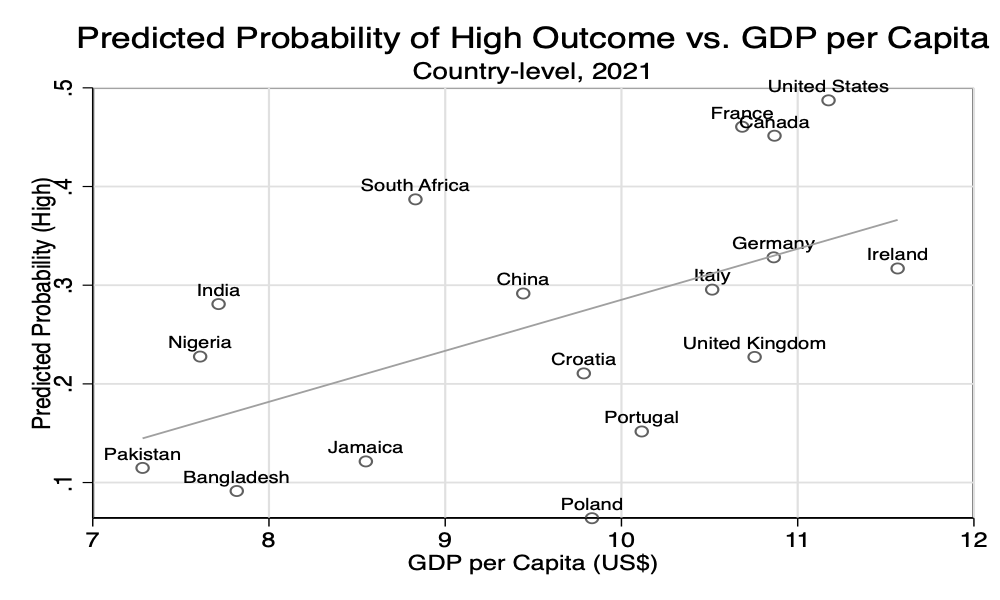
\includegraphics[width=0.5\textwidth]{p_high_vs_gdp.png}  
\caption{Predicted Probability of High Outcome vs. GDP}
\label{fig:high_gdp}
\end{figure}

\begin{figure}[H]
\centering
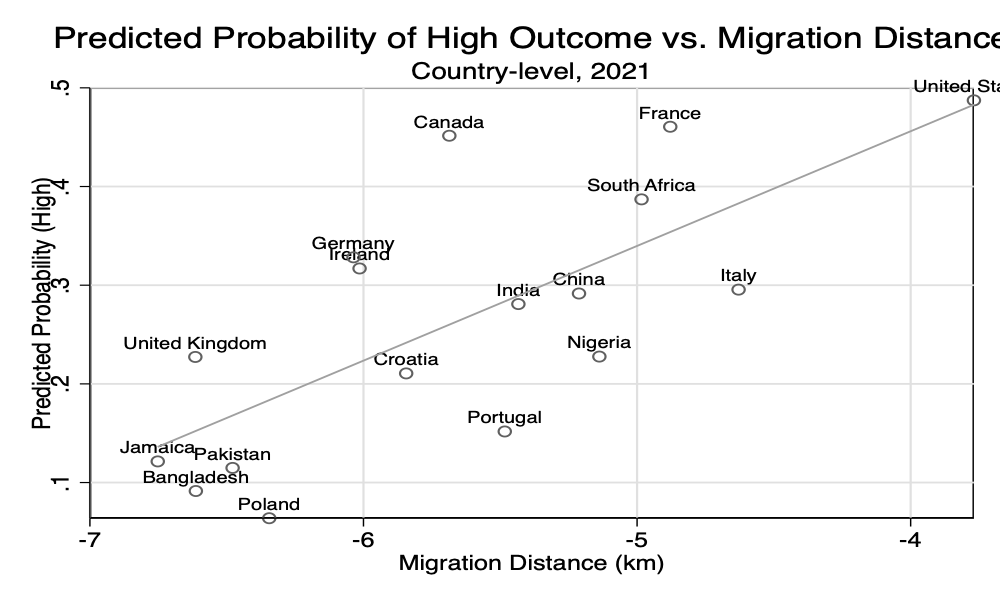
\includegraphics[width=0.5\textwidth]{p_high_vs_dist.png}  
\caption{Predicted Probability of High Outcome vs. Distance}
\label{fig:high_dist}
\end{figure}

\begin{figure}[H]
\centering
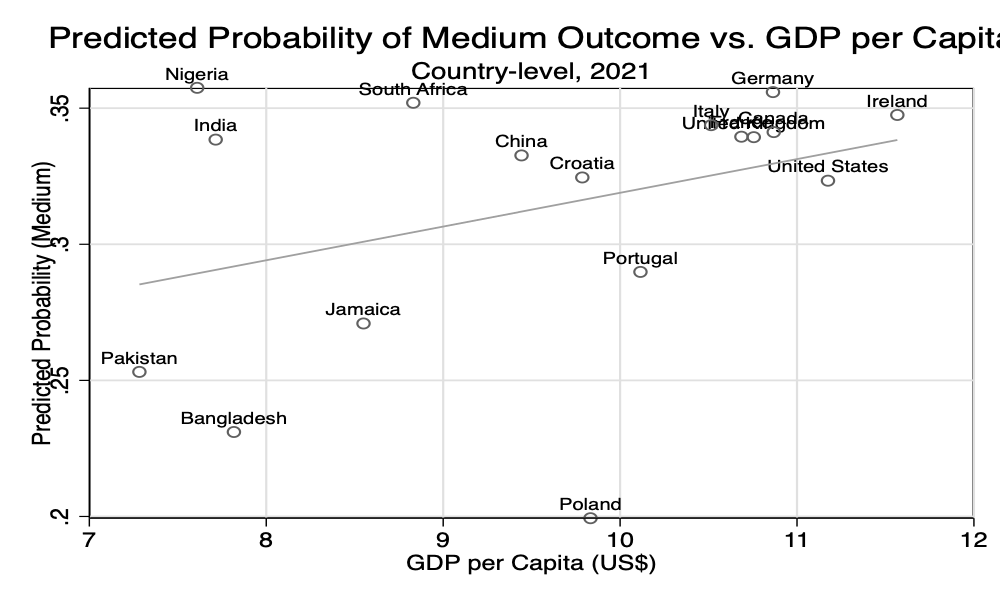
\includegraphics[width=0.5\textwidth]{p_med_vs_gdp.png}  
\caption{Predicted Probability of Medium Outcome vs. GDP}
\label{fig:med_gdp}
\end{figure}

\begin{figure}[H]
\centering
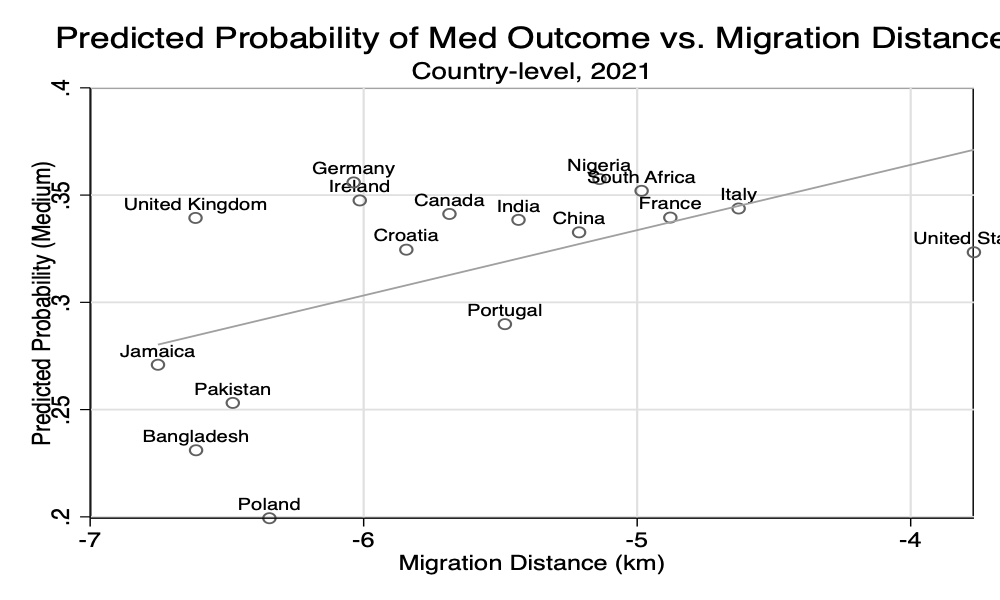
\includegraphics[width=0.5\textwidth]{p_med_vs_dist.png}  
\caption{Predicted Probability of Medium Outcome vs. Distance}
\label{fig:med_dist}
\end{figure}

\begin{figure}[H]
\centering
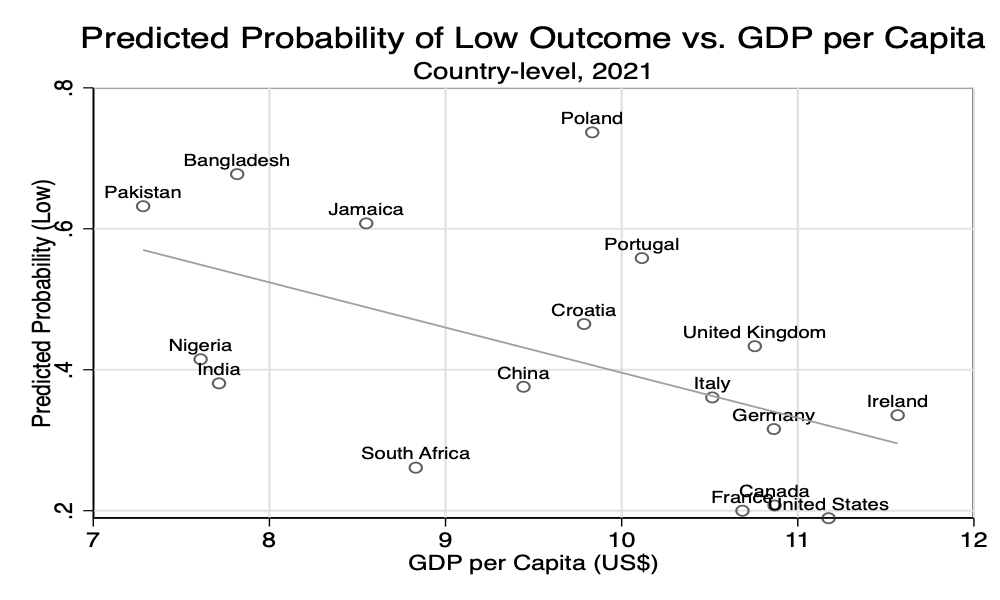
\includegraphics[width=0.5\textwidth]{p_low_vs_gdp.png}  
\caption{Predicted Probability of Low Outcome vs. GDP}
\label{fig:low_gdp}
\end{figure}

\begin{figure}[H]
\centering
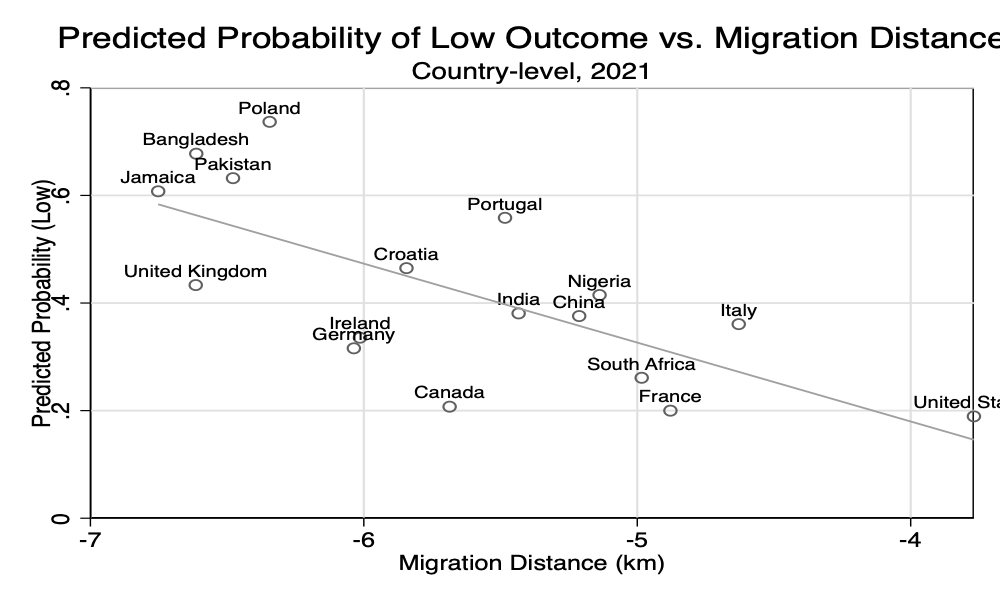
\includegraphics[width=0.5\textwidth]{p_low_vs_dist.png}  
\caption{Predicted Probability of Low Outcome vs. Distance}
\label{fig:low_dist}
\end{figure}

\subsection{Marginal Effects from Multinomial Logit}

\begin{table}[H]
    \centering
        \begin{tabularx}{\textwidth}{@{}lCCC@{}} \hline
         & (1) & (2) & (3) \\
        VARIABLES & High-Skill Logit & Medium-Skill Logit & Low-Skill Logit \\ \hline
         &  &  &  \\
        United Kingdom & 0.204*** & 0.369*** & 0.428*** \\
         & (0.001) & (0.001) & (0.001) \\
        Ireland & 0.231*** & 0.410*** & 0.360*** \\
         & (0.008) & (0.011) & (0.011) \\
        France & 0.300*** & 0.398*** & 0.303*** \\
         & (0.011) & (0.012) & (0.013) \\
        Germany & 0.260*** & 0.385*** & 0.355*** \\
         & (0.008) & (0.009) & (0.009) \\
        Italy & 0.214*** & 0.385*** & 0.401*** \\
         & (0.008) & (0.010) & (0.011) \\
        Portugal & 0.149*** & 0.330*** & 0.520*** \\
         & (0.008) & (0.012) & (0.013) \\
        Poland & 0.068*** & 0.222*** & 0.710*** \\
         & (0.003) & (0.006) & (0.006) \\
        Croatia & 0.179*** & 0.324*** & 0.497*** \\
         & (0.028) & (0.039) & (0.043) \\
        Nigeria & 0.112*** & 0.363*** & 0.525*** \\
         & (0.005) & (0.010) & (0.010) \\
        South Africa & 0.279*** & 0.434*** & 0.288*** \\
         & (0.009) & (0.010) & (0.010) \\
        China & 0.272*** & 0.251*** & 0.477*** \\
         & (0.012) & (0.013) & (0.016) \\
        Bangladesh & 0.076*** & 0.270*** & 0.655*** \\
         & (0.004) & (0.009) & (0.009) \\
        India & 0.219*** & 0.328*** & 0.453*** \\
         & (0.005) & (0.006) & (0.007) \\
        Pakistan & 0.123*** & 0.264*** & 0.613*** \\
         & (0.004) & (0.006) & (0.007) \\
        Canada & 0.310*** & 0.389*** & 0.302*** \\
         & (0.016) & (0.018) & (0.019) \\
        United States & 0.324*** & 0.466*** & 0.210*** \\
         & (0.011) & (0.013) & (0.011) \\
        Jamaica & 0.101*** & 0.388*** & 0.511*** \\
         & (0.009) & (0.016) & (0.017) \\
         &  &  &  \\
         Observations & 516,746 & 516,746 & 516,746 \\ \hline
        \multicolumn{4}{c}{ Standard errors in parentheses} \\
        \multicolumn{4}{c}{ *** p$<$0.01, ** p$<$0.05, * p$<$0.1} \\
        \end{tabularx}
    \caption{Margins from multinomial logit}
    \label{tab:marginsmultinomial}
\end{table}



\subsection{Second-Stage Multinomial}

\begin{table}[H]
    \centering
        \begin{tabularx}{\textwidth}{@{}lCCC@{}} \hline
         & (1) & (2) & (3) \\
        VARIABLES & High-Base & Medium-Base & Low-Base \\ \hline
         &  &  &  \\
        Log GDP per capita, 2021 (US\$) & 0.031** & 0.015 & -0.047** \\
         & (0.012) & (0.010) & (0.016) \\
        Migration distance to UK, 2019 (km) & 0.100*** & 0.027 & -0.127*** \\
         & (0.021) & (0.018) & (0.031) \\
        Constant & 0.541** & 0.293 & 0.166 \\
         & (0.191) & (0.185) & (0.286) \\
         &  &  &  \\
        Observations & 17 & 17 & 17 \\
         R-squared & 0.630 & 0.292 & 0.613 \\ \hline
        \multicolumn{4}{c}{ Robust standard errors in parentheses} \\
        \multicolumn{4}{c}{ *** p$<$0.01, ** p$<$0.05, * p$<$0.1} \\
        \end{tabularx}
    \caption{Second-stage country-level effects from multinomial model - base}
    \label{tab:seconstagemulti_base}
\end{table}


\begin{table}[H]
    \centering
        \begin{tabularx}{\textwidth}{@{}lCCC@{}} \hline
         & (1) & (2) & (3) \\
        VARIABLES & High-Home & Medium-Home & Low-Home \\ \hline
         &  &  &  \\
        Log GDP per capita, 2021 (US\$) & 0.041** & 0.021** & -0.061*** \\
         & (0.016) & (0.009) & (0.016) \\
        Migration distance to UK, 2019 (km) & 0.099*** & 0.035* & -0.134*** \\
         & (0.028) & (0.018) & (0.039) \\
        Home Language - English (Manually encoded) & 0.063 & 0.063** & -0.127* \\
         & (0.051) & (0.025) & (0.060) \\
        Constant & 0.411 & 0.245 & 0.344 \\
         & (0.254) & (0.161) & (0.263) \\
         &  &  &  \\
        Observations & 16 & 16 & 16 \\
         R-squared & 0.675 & 0.550 & 0.734 \\ \hline
        \multicolumn{4}{c}{ Robust standard errors in parentheses} \\
        \multicolumn{4}{c}{ *** p$<$0.01, ** p$<$0.05, * p$<$0.1} \\
        \end{tabularx}
    \caption{Second-stage country-level effects from multinomial model - home}
    \label{tab:seconstagemulti_home}
\end{table}

\subsection{Marginal Effects: Pre and Post-Brexit}

\begin{table}[H]
    \centering
        \begin{tabularx}{\textwidth}{@{}lCCC@{}} \hline
         & (1) & (2) & (3) \\
        VARIABLES & High-Skill Pre & Medium-Skill Pre & Low-Skill Pre \\ \hline
         &  &  &  \\
        United Kingdom & 0.195*** & 0.380*** & 0.425*** \\
         & (0.001) & (0.001) & (0.001) \\
        Ireland & 0.237*** & 0.393*** & 0.370*** \\
         & (0.008) & (0.002) & (0.009) \\
        France & 0.298*** & 0.400*** & 0.302*** \\
         & (0.011) & (0.001) & (0.011) \\
        Germany & 0.247*** & 0.395*** & 0.358*** \\
         & (0.007) & (0.001) & (0.008) \\
        Italy & 0.223*** & 0.390*** & 0.387*** \\
         & (0.007) & (0.002) & (0.010) \\
        Portugal & 0.141*** & 0.348*** & 0.510*** \\
         & (0.007) & (0.005) & (0.012) \\
        Poland & 0.061*** & 0.248*** & 0.691*** \\
         & (0.002) & (0.004) & (0.006) \\
        Croatia & 0.141*** & 0.348*** & 0.511*** \\
         & (0.025) & (0.020) & (0.045) \\
        Nigeria & 0.121*** & 0.331*** & 0.548*** \\
         & (0.005) & (0.005) & (0.009) \\
        South Africa & 0.291*** & 0.400*** & 0.309*** \\
         & (0.008) & (0.001) & (0.008) \\
        China & 0.201*** & 0.382*** & 0.417*** \\
         & (0.010) & (0.004) & (0.014) \\
        Bangladesh & 0.079*** & 0.279*** & 0.642*** \\
         & (0.004) & (0.005) & (0.009) \\
        India & 0.191*** & 0.378*** & 0.431*** \\
         & (0.004) & (0.002) & (0.006) \\
        Pakistan & 0.104*** & 0.313*** & 0.583*** \\
         & (0.003) & (0.004) & (0.007) \\
        Canada & 0.298*** & 0.400*** & 0.302*** \\
         & (0.015) & (0.001) & (0.015) \\
        United States & 0.334*** & 0.398*** & 0.268*** \\
         & (0.012) & (0.001) & (0.011) \\
        Jamaica & 0.124*** & 0.333*** & 0.543*** \\
         & (0.008) & (0.007) & (0.015) \\
         &  &  &  \\
         Observations & 506,608 & 506,608 & 506,608 \\ \hline
        \multicolumn{4}{c}{ Standard errors in parentheses} \\
        \multicolumn{4}{c}{ *** p$<$0.01, ** p$<$0.05, * p$<$0.1} \\
        \end{tabularx}
    \caption{Margins from Pre-Brexit Probit}
    \label{tab:margins_prebrexit}
\end{table}

\begin{table}[H]
    \centering
        \begin{tabularx}{\textwidth}{@{}lCCC@{}} \hline
         & (1) & (2) & (3) \\
        VARIABLES & High-Skill Post & Medium-Skill Post & Low-Skill Post \\ \hline
         &  &  &  \\
        United Kingdom & 0.192*** & 0.382*** & 0.426*** \\
         & (0.001) & (0.001) & (0.001) \\
        Ireland & 0.457*** & 0.372*** & 0.171*** \\
         & (0.036) & (0.013) & (0.023) \\
        France & 0.507*** & 0.352*** & 0.141*** \\
         & (0.028) & (0.012) & (0.016) \\
        Germany & 0.582*** & 0.315*** & 0.103*** \\
         & (0.035) & (0.019) & (0.016) \\
        Italy & 0.355*** & 0.399*** & 0.246*** \\
         & (0.023) & (0.004) & (0.019) \\
        Portugal & 0.274*** & 0.402*** & 0.324*** \\
         & (0.026) & (0.002) & (0.028) \\
        Poland & 0.158*** & 0.364*** & 0.477*** \\
         & (0.016) & (0.010) & (0.026) \\
        Croatia & 0.387*** & 0.393*** & 0.221*** \\
         & (0.062) & (0.014) & (0.048) \\
        Nigeria & 0.277*** & 0.403*** & 0.320*** \\
         & (0.023) & (0.002) & (0.025) \\
        South Africa & 0.517*** & 0.348*** & 0.136*** \\
         & (0.027) & (0.012) & (0.015) \\
        China & 0.506*** & 0.353*** & 0.142*** \\
         & (0.033) & (0.014) & (0.019) \\
        Bangladesh & 0.133*** & 0.345*** & 0.522*** \\
         & (0.018) & (0.015) & (0.033) \\
        India & 0.414*** & 0.386*** & 0.200*** \\
         & (0.020) & (0.006) & (0.015) \\
        Pakistan & 0.235*** & 0.396*** & 0.369*** \\
         & (0.019) & (0.004) & (0.023) \\
        Canada & 0.600*** & 0.305*** & 0.095*** \\
         & (0.046) & (0.026) & (0.020) \\
        United States & 0.584*** & 0.314*** & 0.102*** \\
         & (0.025) & (0.014) & (0.012) \\
        Jamaica & 0.372*** & 0.396*** & 0.232*** \\
         & (0.055) & (0.011) & (0.044) \\
         &  &  &  \\
         Observations & 462,204 & 462,204 & 462,204 \\ \hline
        \multicolumn{4}{c}{ Standard errors in parentheses} \\
        \multicolumn{4}{c}{ *** p$<$0.01, ** p$<$0.05, * p$<$0.1} \\
        \end{tabularx}
    \caption{Margins from Post-Brexit Probit}
    \label{tab:margins_postbrexit}
\end{table}


\subsection{Women}

\begin{table}[H]
    \centering
        \begin{tabularx}{\textwidth}{@{}lCCC@{}} \hline
         & (1) & (2) & (3) \\
        VARIABLES & High‐Skill (women) & Medium‐Skill (women) & Low‐Skill (women) \\ \hline
         &  &  &  \\
        United Kingdom & 0.189*** & 0.429*** & 0.383*** \\
         & (0.000704) & (0.000770) & (0.000920) \\
        Ireland & 0.262*** & 0.445*** & 0.293*** \\
         & (0.00745) & (0.000883) & (0.00788) \\
        France & 0.268*** & 0.445*** & 0.287*** \\
         & (0.00835) & (0.000823) & (0.00863) \\
        Germany & 0.234*** & 0.442*** & 0.325*** \\
         & (0.00588) & (0.00128) & (0.00691) \\
        Italy & 0.220*** & 0.439*** & 0.342*** \\
         & (0.00718) & (0.00189) & (0.00891) \\
        Portugal & 0.119*** & 0.382*** & 0.499*** \\
         & (0.00580) & (0.00584) & (0.0116) \\
        Poland & 0.0719*** & 0.318*** & 0.610*** \\
         & (0.00217) & (0.00390) & (0.00603) \\
        Croatia & 0.176*** & 0.423*** & 0.401*** \\
         & (0.0195) & (0.00968) & (0.0291) \\
        Nigeria & 0.126*** & 0.389*** & 0.485*** \\
         & (0.00450) & (0.00418) & (0.00863) \\
        South Africa & 0.281*** & 0.445*** & 0.274*** \\
         & (0.00746) & (0.000781) & (0.00736) \\
        China & 0.230*** & 0.441*** & 0.328*** \\
         & (0.00838) & (0.00176) & (0.00996) \\
        Bangladesh & 0.109*** & 0.371*** & 0.519*** \\
         & (0.00589) & (0.00666) & (0.0125) \\
        India & 0.201*** & 0.433*** & 0.366*** \\
         & (0.00440) & (0.00167) & (0.00590) \\
        Pakistan & 0.164*** & 0.416*** & 0.420*** \\
         & (0.00533) & (0.00317) & (0.00842) \\
        Canada & 0.294*** & 0.445*** & 0.261*** \\
         & (0.0119) & (0.00103) & (0.0113) \\
        United States & 0.320*** & 0.442*** & 0.238*** \\
         & (0.00906) & (0.00144) & (0.00784) \\
        Jamaica & 0.0974*** & 0.357*** & 0.546*** \\
         & (0.00530) & (0.00691) & (0.0122) \\
         &  &  &  \\
         Observations & 476,288 & 476,288 & 476,288 \\ \hline
        \multicolumn{4}{c}{ Standard errors in parentheses} \\
        \multicolumn{4}{c}{ *** p$<$0.01, ** p$<$0.05, * p$<$0.1} \\
        \end{tabularx}
    \caption{Marginal effects from probit - Women}
    \label{tab:margins_women}
\end{table}


\end{document}